\documentclass[1p]{elsarticle_modified}
%\bibliographystyle{elsarticle-num}

%\usepackage[colorlinks]{hyperref}
%\usepackage{abbrmath_seonhwa} %\Abb, \Ascr, \Acal ,\Abf, \Afrak
\usepackage{amsfonts}
\usepackage{amssymb}
\usepackage{amsmath}
\usepackage{amsthm}
\usepackage{scalefnt}
\usepackage{amsbsy}
\usepackage{kotex}
\usepackage{caption}
\usepackage{subfig}
\usepackage{color}
\usepackage{graphicx}
\usepackage{xcolor} %% white, black, red, green, blue, cyan, magenta, yellow
\usepackage{float}
\usepackage{setspace}
\usepackage{hyperref}

\usepackage{tikz}
\usetikzlibrary{arrows}

\usepackage{multirow}
\usepackage{array} % fixed length table
\usepackage{hhline}

%%%%%%%%%%%%%%%%%%%%%
\makeatletter
\renewcommand*\env@matrix[1][\arraystretch]{%
	\edef\arraystretch{#1}%
	\hskip -\arraycolsep
	\let\@ifnextchar\new@ifnextchar
	\array{*\c@MaxMatrixCols c}}
\makeatother %https://tex.stackexchange.com/questions/14071/how-can-i-increase-the-line-spacing-in-a-matrix
%%%%%%%%%%%%%%%

\usepackage[normalem]{ulem}

\newcommand{\msout}[1]{\ifmmode\text{\sout{\ensuremath{#1}}}\else\sout{#1}\fi}
%SOURCE: \msout is \stkout macro in https://tex.stackexchange.com/questions/20609/strikeout-in-math-mode

\newcommand{\cancel}[1]{
	\ifmmode
	{\color{red}\msout{#1}}
	\else
	{\color{red}\sout{#1}}
	\fi
}

\newcommand{\add}[1]{
	{\color{blue}\uwave{#1}}
}

\newcommand{\replace}[2]{
	\ifmmode
	{\color{red}\msout{#1}}{\color{blue}\uwave{#2}}
	\else
	{\color{red}\sout{#1}}{\color{blue}\uwave{#2}}
	\fi
}

\newcommand{\Sol}{\mathcal{S}} %segment
\newcommand{\D}{D} %diagram
\newcommand{\A}{\mathcal{A}} %arc


%%%%%%%%%%%%%%%%%%%%%%%%%%%%%5 test

\def\sl{\operatorname{\textup{SL}}(2,\Cbb)}
\def\psl{\operatorname{\textup{PSL}}(2,\Cbb)}
\def\quan{\mkern 1mu \triangleright \mkern 1mu}

\theoremstyle{definition}
\newtheorem{thm}{Theorem}[section]
\newtheorem{prop}[thm]{Proposition}
\newtheorem{lem}[thm]{Lemma}
\newtheorem{ques}[thm]{Question}
\newtheorem{cor}[thm]{Corollary}
\newtheorem{defn}[thm]{Definition}
\newtheorem{exam}[thm]{Example}
\newtheorem{rmk}[thm]{Remark}
\newtheorem{alg}[thm]{Algorithm}

\newcommand{\I}{\sqrt{-1}}
\begin{document}

%\begin{frontmatter}
%
%\title{Boundary parabolic representations of knots up to 8 crossings}
%
%%% Group authors per affiliation:
%\author{Yunhi Cho} 
%\address{Department of Mathematics, University of Seoul, Seoul, Korea}
%\ead{yhcho@uos.ac.kr}
%
%
%\author{Seonhwa Kim} %\fnref{s_kim}}
%\address{Center for Geometry and Physics, Institute for Basic Science, Pohang, 37673, Korea}
%\ead{ryeona17@ibs.re.kr}
%
%\author{Hyuk Kim}
%\address{Department of Mathematical Sciences, Seoul National University, Seoul 08826, Korea}
%\ead{hyukkim@snu.ac.kr}
%
%\author{Seokbeom Yoon}
%\address{Department of Mathematical Sciences, Seoul National University, Seoul, 08826,  Korea}
%\ead{sbyoon15@snu.ac.kr}
%
%\begin{abstract}
%We find all boundary parabolic representation of knots up to 8 crossings.
%
%\end{abstract}
%\begin{keyword}
%    \MSC[2010] 57M25 
%\end{keyword}
%
%\end{frontmatter}

%\linenumbers
%\tableofcontents
%
\newcommand\colored[1]{\textcolor{white}{\rule[-0.35ex]{0.8em}{1.4ex}}\kern-0.8em\color{red} #1}%
%\newcommand\colored[1]{\textcolor{white}{ #1}\kern-2.17ex	\textcolor{white}{ #1}\kern-1.81ex	\textcolor{white}{ #1}\kern-2.15ex\color{red}#1	}

{\Large $\underline{12a_{0642}~(K12a_{0642})}$}

\setlength{\tabcolsep}{10pt}
\renewcommand{\arraystretch}{1.6}
\vspace{1cm}\begin{tabular}{m{100pt}>{\centering\arraybackslash}m{274pt}}
\multirow{5}{120pt}{
	\centering
	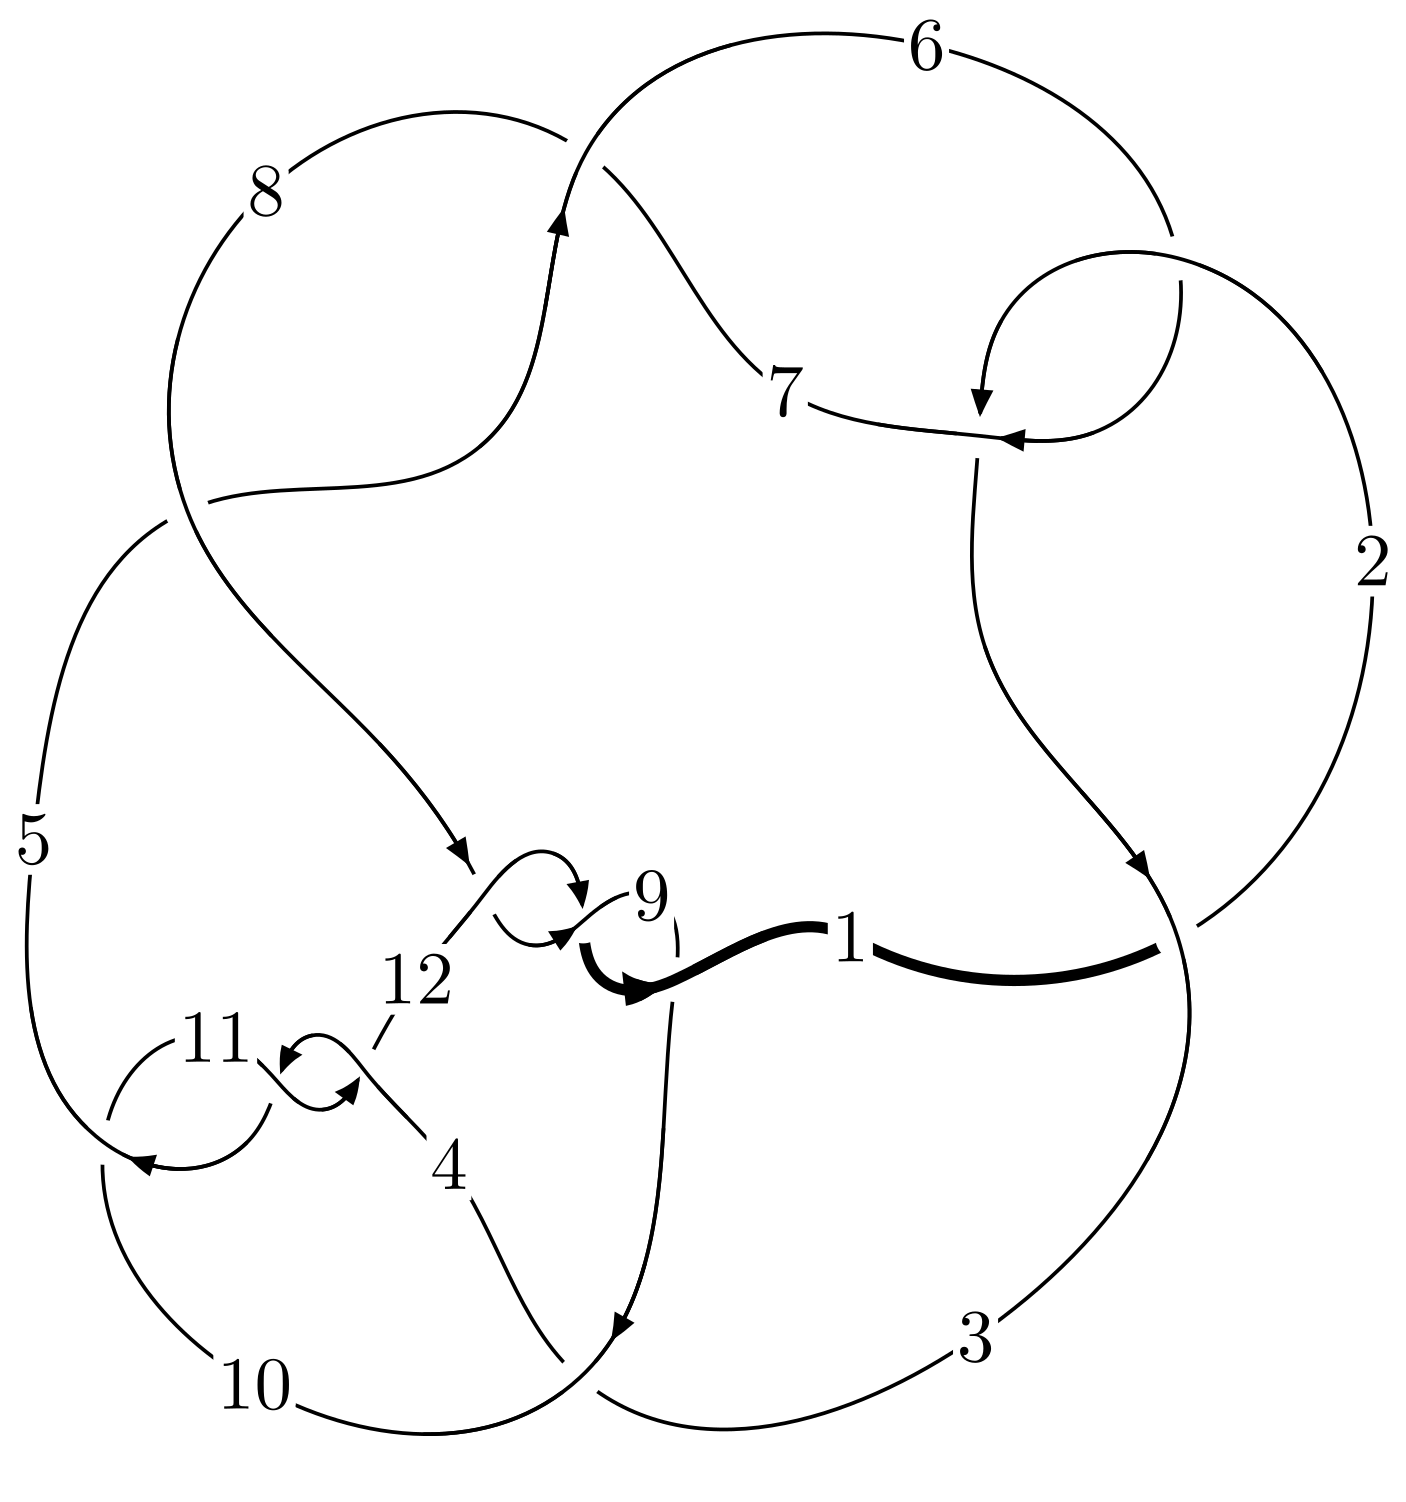
\includegraphics[width=112pt]{../../../GIT/diagram.site/Diagrams/png/1443_12a_0642.png}\\
\ \ \ A knot diagram\footnotemark}&
\allowdisplaybreaks
\textbf{Linearized knot diagam} \\
\cline{2-2}
 &
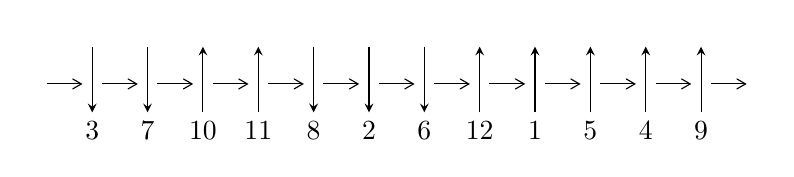
\begin{tikzpicture}[x=20pt, y=17pt]
	% nodes
	\node (C0) at (0, 0) {};
	\node (C1) at (1, 0) {};
	\node (C1U) at (1, +1) {};
	\node (C1D) at (1, -1) {3};

	\node (C2) at (2, 0) {};
	\node (C2U) at (2, +1) {};
	\node (C2D) at (2, -1) {7};

	\node (C3) at (3, 0) {};
	\node (C3U) at (3, +1) {};
	\node (C3D) at (3, -1) {10};

	\node (C4) at (4, 0) {};
	\node (C4U) at (4, +1) {};
	\node (C4D) at (4, -1) {11};

	\node (C5) at (5, 0) {};
	\node (C5U) at (5, +1) {};
	\node (C5D) at (5, -1) {8};

	\node (C6) at (6, 0) {};
	\node (C6U) at (6, +1) {};
	\node (C6D) at (6, -1) {2};

	\node (C7) at (7, 0) {};
	\node (C7U) at (7, +1) {};
	\node (C7D) at (7, -1) {6};

	\node (C8) at (8, 0) {};
	\node (C8U) at (8, +1) {};
	\node (C8D) at (8, -1) {12};

	\node (C9) at (9, 0) {};
	\node (C9U) at (9, +1) {};
	\node (C9D) at (9, -1) {1};

	\node (C10) at (10, 0) {};
	\node (C10U) at (10, +1) {};
	\node (C10D) at (10, -1) {5};

	\node (C11) at (11, 0) {};
	\node (C11U) at (11, +1) {};
	\node (C11D) at (11, -1) {4};

	\node (C12) at (12, 0) {};
	\node (C12U) at (12, +1) {};
	\node (C12D) at (12, -1) {9};
	\node (C13) at (13, 0) {};

	% arrows
	\draw[->,>={angle 60}]
	(C0) edge (C1) (C1) edge (C2) (C2) edge (C3) (C3) edge (C4) (C4) edge (C5) (C5) edge (C6) (C6) edge (C7) (C7) edge (C8) (C8) edge (C9) (C9) edge (C10) (C10) edge (C11) (C11) edge (C12) (C12) edge (C13) ;	\draw[->,>=stealth]
	(C1U) edge (C1D) (C2U) edge (C2D) (C3D) edge (C3U) (C4D) edge (C4U) (C5U) edge (C5D) (C6U) edge (C6D) (C7U) edge (C7D) (C8D) edge (C8U) (C9D) edge (C9U) (C10D) edge (C10U) (C11D) edge (C11U) (C12D) edge (C12U) ;
	\end{tikzpicture} \\
\hhline{~~} \\& 
\textbf{Solving Sequence} \\ \cline{2-2} 
 &
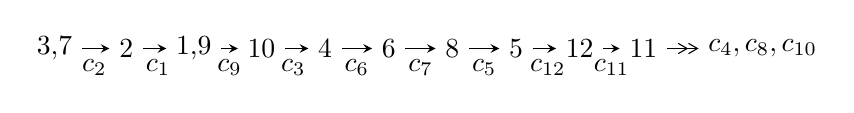
\begin{tikzpicture}[x=23pt, y=7pt]
	% node
	\node (A0) at (-1/8, 0) {3,7};
	\node (A1) at (1, 0) {2};
	\node (A2) at (33/16, 0) {1,9};
	\node (A3) at (25/8, 0) {10};
	\node (A4) at (33/8, 0) {4};
	\node (A5) at (41/8, 0) {6};
	\node (A6) at (49/8, 0) {8};
	\node (A7) at (57/8, 0) {5};
	\node (A8) at (65/8, 0) {12};
	\node (A9) at (73/8, 0) {11};
	\node (C1) at (1/2, -1) {$c_{2}$};
	\node (C2) at (3/2, -1) {$c_{1}$};
	\node (C3) at (21/8, -1) {$c_{9}$};
	\node (C4) at (29/8, -1) {$c_{3}$};
	\node (C5) at (37/8, -1) {$c_{6}$};
	\node (C6) at (45/8, -1) {$c_{7}$};
	\node (C7) at (53/8, -1) {$c_{5}$};
	\node (C8) at (61/8, -1) {$c_{12}$};
	\node (C9) at (69/8, -1) {$c_{11}$};
	\node (A10) at (11, 0) {$c_{4},c_{8},c_{10}$};

	% edge
	\draw[->,>=stealth]	
	(A0) edge (A1) (A1) edge (A2) (A2) edge (A3) (A3) edge (A4) (A4) edge (A5) (A5) edge (A6) (A6) edge (A7) (A7) edge (A8) (A8) edge (A9) ;
	\draw[->>,>={angle 60}]	
	(A9) edge (A10);
\end{tikzpicture} \\ 

\end{tabular} \\

\footnotetext{
The image of knot diagram is generated by the software ``\textbf{Draw programme}" developed by Andrew Bartholomew(\url{http://www.layer8.co.uk/maths/draw/index.htm\#Running-draw}), where we modified some parts for our purpose(\url{https://github.com/CATsTAILs/LinksPainter}).
}\phantom \\ \newline 
\centering \textbf{Ideals for irreducible components\footnotemark of $X_{\text{par}}$} 
 
\begin{align*}
I^u_{1}&=\langle 
-2.08528\times10^{21} u^{65}+3.42453\times10^{21} u^{64}+\cdots+2.45923\times10^{21} b-6.71501\times10^{21},\\
\phantom{I^u_{1}}&\phantom{= \langle  }-7.92933\times10^{20} u^{65}+2.33303\times10^{21} u^{64}+\cdots+7.37769\times10^{21} a-1.03514\times10^{21},\;u^{66}-2 u^{65}+\cdots+5 u-3\rangle \\
I^u_{2}&=\langle 
- u^2+b,\;- u^2+a- u,\;u^3+u^2-1\rangle \\
I^u_{3}&=\langle 
u^2 a- a u+u^2+b- u+1,\;2 u^2 a+a^2-2 a u+2 u^2- u+1,\;u^3- u^2+1\rangle \\
\\
\end{align*}
\raggedright * 3 irreducible components of $\dim_{\mathbb{C}}=0$, with total 75 representations.\\
\footnotetext{All coefficients of polynomials are rational numbers. But the coefficients are sometimes approximated in decimal forms when there is not enough margin.}
\newpage
\renewcommand{\arraystretch}{1}
\centering \section*{I. $I^u_{1}= \langle -2.09\times10^{21} u^{65}+3.42\times10^{21} u^{64}+\cdots+2.46\times10^{21} b-6.72\times10^{21},\;-7.93\times10^{20} u^{65}+2.33\times10^{21} u^{64}+\cdots+7.38\times10^{21} a-1.04\times10^{21},\;u^{66}-2 u^{65}+\cdots+5 u-3 \rangle$}
\flushleft \textbf{(i) Arc colorings}\\
\begin{tabular}{m{7pt} m{180pt} m{7pt} m{180pt} }
\flushright $a_{3}=$&$\begin{pmatrix}1\\0\end{pmatrix}$ \\
\flushright $a_{7}=$&$\begin{pmatrix}0\\u\end{pmatrix}$ \\
\flushright $a_{2}=$&$\begin{pmatrix}1\\- u^2\end{pmatrix}$ \\
\flushright $a_{1}=$&$\begin{pmatrix}- u^2+1\\- u^2\end{pmatrix}$ \\
\flushright $a_{9}=$&$\begin{pmatrix}0.107477 u^{65}-0.316227 u^{64}+\cdots+4.20310 u+0.140307\\0.847942 u^{65}-1.39252 u^{64}+\cdots+1.15079 u+2.73053\end{pmatrix}$ \\
\flushright $a_{10}=$&$\begin{pmatrix}-0.116848 u^{65}+0.169205 u^{64}+\cdots+7.20302 u-0.938417\\-0.135801 u^{65}-0.253372 u^{64}+\cdots+3.19813 u+0.135182\end{pmatrix}$ \\
\flushright $a_{4}=$&$\begin{pmatrix}0.435419 u^{65}-0.831909 u^{64}+\cdots-2.53069 u+0.102436\\-0.849654 u^{65}+0.956704 u^{64}+\cdots+1.71311 u-2.32719\end{pmatrix}$ \\
\flushright $a_{6}=$&$\begin{pmatrix}u\\- u^3+u\end{pmatrix}$ \\
\flushright $a_{8}=$&$\begin{pmatrix}- u^3\\u^5- u^3+u\end{pmatrix}$ \\
\flushright $a_{5}=$&$\begin{pmatrix}u^5+u\\- u^7+u^5-2 u^3+u\end{pmatrix}$ \\
\flushright $a_{12}=$&$\begin{pmatrix}0.808905 u^{65}-0.823841 u^{64}+\cdots-1.79298 u+6.02411\\-0.647456 u^{65}+0.938023 u^{64}+\cdots+1.14605 u-2.05947\end{pmatrix}$ \\
\flushright $a_{11}=$&$\begin{pmatrix}-0.228635 u^{65}+0.368246 u^{64}+\cdots+5.73814 u-0.217095\\0.0421408 u^{65}-0.505020 u^{64}+\cdots+2.54989 u+1.29366\end{pmatrix}$\\&\end{tabular}
\flushleft \textbf{(ii) Obstruction class $= -1$}\\~\\
\flushleft \textbf{(iii) Cusp Shapes $= \frac{6130397275329191743669}{1229615623032466676507} u^{65}-\frac{9723677310654894627572}{1229615623032466676507} u^{64}+\cdots+\frac{20879266412996566941410}{1229615623032466676507} u+\frac{23149949036627936894973}{1229615623032466676507}$}\\~\\
\newpage\renewcommand{\arraystretch}{1}
\flushleft \textbf{(iv) u-Polynomials at the component}\newline \\
\begin{tabular}{m{50pt}|m{274pt}}
Crossings & \hspace{64pt}u-Polynomials at each crossing \\
\hline $$\begin{aligned}c_{1},c_{5},c_{7}\end{aligned}$$&$\begin{aligned}
&u^{66}+16 u^{65}+\cdots+151 u+9
\end{aligned}$\\
\hline $$\begin{aligned}c_{2},c_{6}\end{aligned}$$&$\begin{aligned}
&u^{66}-2 u^{65}+\cdots+5 u-3
\end{aligned}$\\
\hline $$\begin{aligned}c_{3}\end{aligned}$$&$\begin{aligned}
&u^{66}+u^{65}+\cdots+1808 u+1480
\end{aligned}$\\
\hline $$\begin{aligned}c_{4},c_{10},c_{11}\end{aligned}$$&$\begin{aligned}
&u^{66}- u^{65}+\cdots-32 u+8
\end{aligned}$\\
\hline $$\begin{aligned}c_{8},c_{9},c_{12}\end{aligned}$$&$\begin{aligned}
&u^{66}-4 u^{65}+\cdots-12 u-1
\end{aligned}$\\
\hline
\end{tabular}\\~\\
\newpage\renewcommand{\arraystretch}{1}
\flushleft \textbf{(v) Riley Polynomials at the component}\newline \\
\begin{tabular}{m{50pt}|m{274pt}}
Crossings & \hspace{64pt}Riley Polynomials at each crossing \\
\hline $$\begin{aligned}c_{1},c_{5},c_{7}\end{aligned}$$&$\begin{aligned}
&y^{66}+72 y^{65}+\cdots+1949 y+81
\end{aligned}$\\
\hline $$\begin{aligned}c_{2},c_{6}\end{aligned}$$&$\begin{aligned}
&y^{66}-16 y^{65}+\cdots-151 y+9
\end{aligned}$\\
\hline $$\begin{aligned}c_{3}\end{aligned}$$&$\begin{aligned}
&y^{66}-25 y^{65}+\cdots+8713216 y+2190400
\end{aligned}$\\
\hline $$\begin{aligned}c_{4},c_{10},c_{11}\end{aligned}$$&$\begin{aligned}
&y^{66}+59 y^{65}+\cdots-128 y+64
\end{aligned}$\\
\hline $$\begin{aligned}c_{8},c_{9},c_{12}\end{aligned}$$&$\begin{aligned}
&y^{66}-66 y^{65}+\cdots+210 y+1
\end{aligned}$\\
\hline
\end{tabular}\\~\\
\newpage\flushleft \textbf{(vi) Complex Volumes and Cusp Shapes}
$$\begin{array}{c|c|c}  
\text{Solutions to }I^u_{1}& \I (\text{vol} + \sqrt{-1}CS) & \text{Cusp shape}\\
 \hline 
\begin{aligned}
u &= -0.940880 + 0.389587 I \\
a &= \phantom{-}0.801166 - 0.701373 I \\
b &= \phantom{-}0.261406 + 0.593445 I\end{aligned}
 & -5.12964 + 6.16163 I & -3.04372 - 8.05147 I \\ \hline\begin{aligned}
u &= -0.940880 - 0.389587 I \\
a &= \phantom{-}0.801166 + 0.701373 I \\
b &= \phantom{-}0.261406 - 0.593445 I\end{aligned}
 & -5.12964 - 6.16163 I & -3.04372 + 8.05147 I \\ \hline\begin{aligned}
u &= -1.02149\phantom{ +0.000000I} \\
a &= -1.32124\phantom{ +0.000000I} \\
b &= -0.413413\phantom{ +0.000000I}\end{aligned}
 & \phantom{-}2.55529\phantom{ +0.000000I} & \phantom{-}4.40390\phantom{ +0.000000I} \\ \hline\begin{aligned}
u &= -0.796362 + 0.550324 I \\
a &= -0.924966 - 0.099092 I \\
b &= \phantom{-}0.43221 - 1.57388 I\end{aligned}
 & \phantom{-}3.14358 + 2.21788 I & \phantom{-}4.13427 - 2.24025 I \\ \hline\begin{aligned}
u &= -0.796362 - 0.550324 I \\
a &= -0.924966 + 0.099092 I \\
b &= \phantom{-}0.43221 + 1.57388 I\end{aligned}
 & \phantom{-}3.14358 - 2.21788 I & \phantom{-}4.13427 + 2.24025 I \\ \hline\begin{aligned}
u &= \phantom{-}1.046540 + 0.097833 I \\
a &= \phantom{-}1.322190 - 0.020742 I \\
b &= \phantom{-}0.397058 - 0.080498 I\end{aligned}
 & -1.46918 + 3.46747 I & \phantom{-0.000000 } 0 \\ \hline\begin{aligned}
u &= \phantom{-}1.046540 - 0.097833 I \\
a &= \phantom{-}1.322190 + 0.020742 I \\
b &= \phantom{-}0.397058 + 0.080498 I\end{aligned}
 & -1.46918 - 3.46747 I & \phantom{-0.000000 } 0 \\ \hline\begin{aligned}
u &= \phantom{-}0.921469 + 0.129566 I \\
a &= -0.661877 - 0.412132 I \\
b &= \phantom{-}0.514033 + 0.681154 I\end{aligned}
 & -6.59268 + 0.97290 I & -7.57653 - 0.39847 I \\ \hline\begin{aligned}
u &= \phantom{-}0.921469 - 0.129566 I \\
a &= -0.661877 + 0.412132 I \\
b &= \phantom{-}0.514033 - 0.681154 I\end{aligned}
 & -6.59268 - 0.97290 I & -7.57653 + 0.39847 I \\ \hline\begin{aligned}
u &= \phantom{-}0.833726 + 0.384546 I \\
a &= -0.587442 - 0.795014 I \\
b &= -0.144390 + 0.286926 I\end{aligned}
 & -0.18506 - 3.20503 I & \phantom{-}2.36874 + 8.90166 I\\
 \hline 
 \end{array}$$\newpage$$\begin{array}{c|c|c}  
\text{Solutions to }I^u_{1}& \I (\text{vol} + \sqrt{-1}CS) & \text{Cusp shape}\\
 \hline 
\begin{aligned}
u &= \phantom{-}0.833726 - 0.384546 I \\
a &= -0.587442 + 0.795014 I \\
b &= -0.144390 - 0.286926 I\end{aligned}
 & -0.18506 + 3.20503 I & \phantom{-}2.36874 - 8.90166 I \\ \hline\begin{aligned}
u &= \phantom{-}0.990925 + 0.475204 I \\
a &= \phantom{-}0.428686 + 0.120652 I \\
b &= -0.10012 - 1.70913 I\end{aligned}
 & \phantom{-}5.36492 - 5.88722 I & \phantom{-0.000000 } 0 \\ \hline\begin{aligned}
u &= \phantom{-}0.990925 - 0.475204 I \\
a &= \phantom{-}0.428686 - 0.120652 I \\
b &= -0.10012 + 1.70913 I\end{aligned}
 & \phantom{-}5.36492 + 5.88722 I & \phantom{-0.000000 } 0 \\ \hline\begin{aligned}
u &= -0.498795 + 0.739168 I \\
a &= -1.153080 - 0.711498 I \\
b &= \phantom{-}0.622959 - 1.122100 I\end{aligned}
 & \phantom{-}4.16450 + 2.72632 I & \phantom{-}6.92245 - 3.37892 I \\ \hline\begin{aligned}
u &= -0.498795 - 0.739168 I \\
a &= -1.153080 + 0.711498 I \\
b &= \phantom{-}0.622959 + 1.122100 I\end{aligned}
 & \phantom{-}4.16450 - 2.72632 I & \phantom{-}6.92245 + 3.37892 I \\ \hline\begin{aligned}
u &= -1.029240 + 0.415785 I \\
a &= -0.304326 + 0.230817 I \\
b &= \phantom{-}0.01201 - 1.76238 I\end{aligned}
 & \phantom{-}0.44075 + 9.86566 I & \phantom{-0.000000 } 0 \\ \hline\begin{aligned}
u &= -1.029240 - 0.415785 I \\
a &= -0.304326 - 0.230817 I \\
b &= \phantom{-}0.01201 + 1.76238 I\end{aligned}
 & \phantom{-}0.44075 - 9.86566 I & \phantom{-0.000000 } 0 \\ \hline\begin{aligned}
u &= -0.793049 + 0.384644 I \\
a &= -1.47843 + 0.13514 I \\
b &= -0.776296 - 0.191562 I\end{aligned}
 & -3.25737 + 1.93313 I & \phantom{-}0.42721 - 3.82999 I \\ \hline\begin{aligned}
u &= -0.793049 - 0.384644 I \\
a &= -1.47843 - 0.13514 I \\
b &= -0.776296 + 0.191562 I\end{aligned}
 & -3.25737 - 1.93313 I & \phantom{-}0.42721 + 3.82999 I \\ \hline\begin{aligned}
u &= -0.959975 + 0.624161 I \\
a &= -0.499021 - 0.214013 I \\
b &= \phantom{-}0.15361 - 1.51024 I\end{aligned}
 & \phantom{-}2.82571 + 2.19205 I & \phantom{-0.000000 } 0\\
 \hline 
 \end{array}$$\newpage$$\begin{array}{c|c|c}  
\text{Solutions to }I^u_{1}& \I (\text{vol} + \sqrt{-1}CS) & \text{Cusp shape}\\
 \hline 
\begin{aligned}
u &= -0.959975 - 0.624161 I \\
a &= -0.499021 + 0.214013 I \\
b &= \phantom{-}0.15361 + 1.51024 I\end{aligned}
 & \phantom{-}2.82571 - 2.19205 I & \phantom{-0.000000 } 0 \\ \hline\begin{aligned}
u &= -0.886053 + 0.741340 I \\
a &= -0.89572 - 1.29867 I \\
b &= \phantom{-}0.177451 - 1.335260 I\end{aligned}
 & -1.92250 + 2.81816 I & \phantom{-0.000000 } 0 \\ \hline\begin{aligned}
u &= -0.886053 - 0.741340 I \\
a &= -0.89572 + 1.29867 I \\
b &= \phantom{-}0.177451 + 1.335260 I\end{aligned}
 & -1.92250 - 2.81816 I & \phantom{-0.000000 } 0 \\ \hline\begin{aligned}
u &= \phantom{-}0.882438 + 0.780869 I \\
a &= \phantom{-}0.699653 - 0.793108 I \\
b &= -0.180230 - 1.231910 I\end{aligned}
 & \phantom{-}4.00172 - 2.93689 I & \phantom{-0.000000 } 0 \\ \hline\begin{aligned}
u &= \phantom{-}0.882438 - 0.780869 I \\
a &= \phantom{-}0.699653 + 0.793108 I \\
b &= -0.180230 + 1.231910 I\end{aligned}
 & \phantom{-}4.00172 + 2.93689 I & \phantom{-0.000000 } 0 \\ \hline\begin{aligned}
u &= \phantom{-}0.356962 + 0.735559 I \\
a &= \phantom{-}1.16102 - 0.91617 I \\
b &= -0.668874 - 1.010960 I\end{aligned}
 & \phantom{-}7.41551 + 1.48844 I & \phantom{-}10.63091 - 0.75571 I \\ \hline\begin{aligned}
u &= \phantom{-}0.356962 - 0.735559 I \\
a &= \phantom{-}1.16102 + 0.91617 I \\
b &= -0.668874 + 1.010960 I\end{aligned}
 & \phantom{-}7.41551 - 1.48844 I & \phantom{-}10.63091 + 0.75571 I \\ \hline\begin{aligned}
u &= \phantom{-}0.727878 + 0.303493 I \\
a &= \phantom{-}1.48101 + 0.77779 I \\
b &= -0.88271 - 2.24176 I\end{aligned}
 & -3.78561 - 1.23006 I & \phantom{-}1.98020 + 5.99169 I \\ \hline\begin{aligned}
u &= \phantom{-}0.727878 - 0.303493 I \\
a &= \phantom{-}1.48101 - 0.77779 I \\
b &= -0.88271 + 2.24176 I\end{aligned}
 & -3.78561 + 1.23006 I & \phantom{-}1.98020 - 5.99169 I \\ \hline\begin{aligned}
u &= -0.248411 + 0.746724 I \\
a &= -1.07892 - 1.06631 I \\
b &= \phantom{-}0.658592 - 0.929096 I\end{aligned}
 & \phantom{-}2.98364 - 5.69446 I & \phantom{-}6.38560 + 3.41468 I\\
 \hline 
 \end{array}$$\newpage$$\begin{array}{c|c|c}  
\text{Solutions to }I^u_{1}& \I (\text{vol} + \sqrt{-1}CS) & \text{Cusp shape}\\
 \hline 
\begin{aligned}
u &= -0.248411 - 0.746724 I \\
a &= -1.07892 + 1.06631 I \\
b &= \phantom{-}0.658592 + 0.929096 I\end{aligned}
 & \phantom{-}2.98364 + 5.69446 I & \phantom{-}6.38560 - 3.41468 I \\ \hline\begin{aligned}
u &= -0.762533 + 0.185034 I \\
a &= \phantom{-}0.400057 - 0.427963 I \\
b &= -0.335136 + 0.241912 I\end{aligned}
 & -1.264720 + 0.575310 I & -4.44845 - 0.83683 I \\ \hline\begin{aligned}
u &= -0.762533 - 0.185034 I \\
a &= \phantom{-}0.400057 + 0.427963 I \\
b &= -0.335136 - 0.241912 I\end{aligned}
 & -1.264720 - 0.575310 I & -4.44845 + 0.83683 I \\ \hline\begin{aligned}
u &= \phantom{-}0.849055 + 0.877486 I \\
a &= \phantom{-}0.144726 - 0.873025 I \\
b &= -0.025755 - 1.136960 I\end{aligned}
 & \phantom{-}2.96927 + 3.52515 I & \phantom{-0.000000 } 0 \\ \hline\begin{aligned}
u &= \phantom{-}0.849055 - 0.877486 I \\
a &= \phantom{-}0.144726 + 0.873025 I \\
b &= -0.025755 + 1.136960 I\end{aligned}
 & \phantom{-}2.96927 - 3.52515 I & \phantom{-0.000000 } 0 \\ \hline\begin{aligned}
u &= \phantom{-}0.887168 + 0.853480 I \\
a &= \phantom{-}0.936403 - 0.683518 I \\
b &= -0.229264 - 1.107390 I\end{aligned}
 & \phantom{-}4.14950 - 1.92316 I & \phantom{-0.000000 } 0 \\ \hline\begin{aligned}
u &= \phantom{-}0.887168 - 0.853480 I \\
a &= \phantom{-}0.936403 + 0.683518 I \\
b &= -0.229264 + 1.107390 I\end{aligned}
 & \phantom{-}4.14950 + 1.92316 I & \phantom{-0.000000 } 0 \\ \hline\begin{aligned}
u &= \phantom{-}0.825576 + 0.913463 I \\
a &= -0.59888 + 3.00432 I \\
b &= \phantom{-}1.19791 + 3.03712 I\end{aligned}
 & \phantom{-}9.28839 + 8.00052 I & \phantom{-0.000000 } 0 \\ \hline\begin{aligned}
u &= \phantom{-}0.825576 - 0.913463 I \\
a &= -0.59888 - 3.00432 I \\
b &= \phantom{-}1.19791 - 3.03712 I\end{aligned}
 & \phantom{-}9.28839 - 8.00052 I & \phantom{-0.000000 } 0 \\ \hline\begin{aligned}
u &= -0.884770 + 0.860589 I \\
a &= -0.212411 - 0.810921 I \\
b &= \phantom{-}0.040113 - 1.187130 I\end{aligned}
 & \phantom{-}7.38355 + 0.47295 I & \phantom{-0.000000 } 0\\
 \hline 
 \end{array}$$\newpage$$\begin{array}{c|c|c}  
\text{Solutions to }I^u_{1}& \I (\text{vol} + \sqrt{-1}CS) & \text{Cusp shape}\\
 \hline 
\begin{aligned}
u &= -0.884770 - 0.860589 I \\
a &= -0.212411 + 0.810921 I \\
b &= \phantom{-}0.040113 + 1.187130 I\end{aligned}
 & \phantom{-}7.38355 - 0.47295 I & \phantom{-0.000000 } 0 \\ \hline\begin{aligned}
u &= -0.907494 + 0.841916 I \\
a &= \phantom{-}2.68354 + 3.61420 I \\
b &= -0.25692 + 4.58473 I\end{aligned}
 & \phantom{-}2.86142 + 3.13275 I & \phantom{-0.000000 } 0 \\ \hline\begin{aligned}
u &= -0.907494 - 0.841916 I \\
a &= \phantom{-}2.68354 - 3.61420 I \\
b &= -0.25692 - 4.58473 I\end{aligned}
 & \phantom{-}2.86142 - 3.13275 I & \phantom{-0.000000 } 0 \\ \hline\begin{aligned}
u &= -0.854780 + 0.913777 I \\
a &= \phantom{-}0.95509 + 2.99116 I \\
b &= -0.97675 + 3.23830 I\end{aligned}
 & \phantom{-}14.5393 - 3.2940 I & \phantom{-0.000000 } 0 \\ \hline\begin{aligned}
u &= -0.854780 - 0.913777 I \\
a &= \phantom{-}0.95509 - 2.99116 I \\
b &= -0.97675 - 3.23830 I\end{aligned}
 & \phantom{-}14.5393 + 3.2940 I & \phantom{-0.000000 } 0 \\ \hline\begin{aligned}
u &= \phantom{-}0.928525 + 0.839216 I \\
a &= \phantom{-}0.267321 - 0.699993 I \\
b &= -0.044132 - 1.250160 I\end{aligned}
 & \phantom{-}4.02096 - 4.36836 I & \phantom{-0.000000 } 0 \\ \hline\begin{aligned}
u &= \phantom{-}0.928525 - 0.839216 I \\
a &= \phantom{-}0.267321 + 0.699993 I \\
b &= -0.044132 + 1.250160 I\end{aligned}
 & \phantom{-}4.02096 + 4.36836 I & \phantom{-0.000000 } 0 \\ \hline\begin{aligned}
u &= -0.935049 + 0.841580 I \\
a &= -0.997222 - 0.708350 I \\
b &= \phantom{-}0.164677 - 1.077480 I\end{aligned}
 & \phantom{-}7.22562 + 5.84884 I & \phantom{-0.000000 } 0 \\ \hline\begin{aligned}
u &= -0.935049 - 0.841580 I \\
a &= -0.997222 + 0.708350 I \\
b &= \phantom{-}0.164677 + 1.077480 I\end{aligned}
 & \phantom{-}7.22562 - 5.84884 I & \phantom{-0.000000 } 0 \\ \hline\begin{aligned}
u &= \phantom{-}0.886666 + 0.900213 I \\
a &= -1.43168 + 3.00902 I \\
b &= \phantom{-}0.70096 + 3.51971 I\end{aligned}
 & \phantom{-}12.21740 - 1.91088 I & \phantom{-0.000000 } 0\\
 \hline 
 \end{array}$$\newpage$$\begin{array}{c|c|c}  
\text{Solutions to }I^u_{1}& \I (\text{vol} + \sqrt{-1}CS) & \text{Cusp shape}\\
 \hline 
\begin{aligned}
u &= \phantom{-}0.886666 - 0.900213 I \\
a &= -1.43168 - 3.00902 I \\
b &= \phantom{-}0.70096 - 3.51971 I\end{aligned}
 & \phantom{-}12.21740 + 1.91088 I & \phantom{-0.000000 } 0 \\ \hline\begin{aligned}
u &= \phantom{-}0.965870 + 0.830951 I \\
a &= \phantom{-}1.048900 - 0.703382 I \\
b &= -0.122028 - 1.049300 I\end{aligned}
 & \phantom{-}2.60149 - 9.86130 I & \phantom{-0.000000 } 0 \\ \hline\begin{aligned}
u &= \phantom{-}0.965870 - 0.830951 I \\
a &= \phantom{-}1.048900 + 0.703382 I \\
b &= -0.122028 + 1.049300 I\end{aligned}
 & \phantom{-}2.60149 + 9.86130 I & \phantom{-0.000000 } 0 \\ \hline\begin{aligned}
u &= \phantom{-}0.957311 + 0.866384 I \\
a &= -2.46807 + 2.30758 I \\
b &= -0.30755 + 3.64760 I\end{aligned}
 & \phantom{-}11.99000 - 4.61174 I & \phantom{-0.000000 } 0 \\ \hline\begin{aligned}
u &= \phantom{-}0.957311 - 0.866384 I \\
a &= -2.46807 - 2.30758 I \\
b &= -0.30755 - 3.64760 I\end{aligned}
 & \phantom{-}11.99000 + 4.61174 I & \phantom{-0.000000 } 0 \\ \hline\begin{aligned}
u &= \phantom{-}0.998275 + 0.835366 I \\
a &= -2.75742 + 1.52819 I \\
b &= -0.88652 + 3.29956 I\end{aligned}
 & \phantom{-}8.7382 - 14.4571 I & \phantom{-0.000000 } 0 \\ \hline\begin{aligned}
u &= \phantom{-}0.998275 - 0.835366 I \\
a &= -2.75742 - 1.52819 I \\
b &= -0.88652 - 3.29956 I\end{aligned}
 & \phantom{-}8.7382 + 14.4571 I & \phantom{-0.000000 } 0 \\ \hline\begin{aligned}
u &= -0.983999 + 0.853365 I \\
a &= \phantom{-}2.61145 + 1.85077 I \\
b &= \phantom{-}0.63135 + 3.43344 I\end{aligned}
 & \phantom{-}14.1256 + 9.8142 I & \phantom{-0.000000 } 0 \\ \hline\begin{aligned}
u &= -0.983999 - 0.853365 I \\
a &= \phantom{-}2.61145 - 1.85077 I \\
b &= \phantom{-}0.63135 - 3.43344 I\end{aligned}
 & \phantom{-}14.1256 - 9.8142 I & \phantom{-0.000000 } 0 \\ \hline\begin{aligned}
u &= -0.482668 + 0.473305 I \\
a &= \phantom{-}0.026115 - 1.148390 I \\
b &= -0.243945 - 0.319913 I\end{aligned}
 & -2.37826 + 1.37049 I & \phantom{-}3.17735 - 4.52175 I\\
 \hline 
 \end{array}$$\newpage$$\begin{array}{c|c|c}  
\text{Solutions to }I^u_{1}& \I (\text{vol} + \sqrt{-1}CS) & \text{Cusp shape}\\
 \hline 
\begin{aligned}
u &= -0.482668 - 0.473305 I \\
a &= \phantom{-}0.026115 + 1.148390 I \\
b &= -0.243945 + 0.319913 I\end{aligned}
 & -2.37826 - 1.37049 I & \phantom{-}3.17735 + 4.52175 I \\ \hline\begin{aligned}
u &= -0.268428 + 0.572165 I \\
a &= -0.433288 + 0.777956 I \\
b &= -0.434835 + 0.673053 I\end{aligned}
 & -3.09183 - 2.58712 I & \phantom{-}2.42181 + 3.21581 I \\ \hline\begin{aligned}
u &= -0.268428 - 0.572165 I \\
a &= -0.433288 - 0.777956 I \\
b &= -0.434835 - 0.673053 I\end{aligned}
 & -3.09183 + 2.58712 I & \phantom{-}2.42181 - 3.21581 I \\ \hline\begin{aligned}
u &= \phantom{-}0.438013 + 0.335978 I \\
a &= \phantom{-}0.778089 + 0.240873 I \\
b &= \phantom{-}0.555725 + 0.212651 I\end{aligned}
 & \phantom{-}0.967621 + 0.114990 I & \phantom{-}10.14067 - 0.04829 I \\ \hline\begin{aligned}
u &= \phantom{-}0.438013 - 0.335978 I \\
a &= \phantom{-}0.778089 - 0.240873 I \\
b &= \phantom{-}0.555725 - 0.212651 I\end{aligned}
 & \phantom{-}0.967621 - 0.114990 I & \phantom{-}10.14067 + 0.04829 I \\ \hline\begin{aligned}
u &= \phantom{-}0.493664\phantom{ +0.000000I} \\
a &= \phantom{-}1.46260\phantom{ +0.000000I} \\
b &= \phantom{-}0.604228\phantom{ +0.000000I}\end{aligned}
 & \phantom{-}0.957505\phantom{ +0.000000I} & \phantom{-}14.1910\phantom{ +0.000000I}\\
 \hline 
 \end{array}$$\newpage\newpage\renewcommand{\arraystretch}{1}
\centering \section*{II. $I^u_{2}= \langle - u^2+b,\;- u^2+a- u,\;u^3+u^2-1 \rangle$}
\flushleft \textbf{(i) Arc colorings}\\
\begin{tabular}{m{7pt} m{180pt} m{7pt} m{180pt} }
\flushright $a_{3}=$&$\begin{pmatrix}1\\0\end{pmatrix}$ \\
\flushright $a_{7}=$&$\begin{pmatrix}0\\u\end{pmatrix}$ \\
\flushright $a_{2}=$&$\begin{pmatrix}1\\- u^2\end{pmatrix}$ \\
\flushright $a_{1}=$&$\begin{pmatrix}- u^2+1\\- u^2\end{pmatrix}$ \\
\flushright $a_{9}=$&$\begin{pmatrix}u^2+u\\u^2\end{pmatrix}$ \\
\flushright $a_{10}=$&$\begin{pmatrix}u+1\\0\end{pmatrix}$ \\
\flushright $a_{4}=$&$\begin{pmatrix}1\\0\end{pmatrix}$ \\
\flushright $a_{6}=$&$\begin{pmatrix}u\\u^2+u-1\end{pmatrix}$ \\
\flushright $a_{8}=$&$\begin{pmatrix}u^2-1\\u^2\end{pmatrix}$ \\
\flushright $a_{5}=$&$\begin{pmatrix}1\\0\end{pmatrix}$ \\
\flushright $a_{12}=$&$\begin{pmatrix}u+1\\0\end{pmatrix}$ \\
\flushright $a_{11}=$&$\begin{pmatrix}u+1\\0\end{pmatrix}$\\&\end{tabular}
\flushleft \textbf{(ii) Obstruction class $= 1$}\\~\\
\flushleft \textbf{(iii) Cusp Shapes $= -4 u^2-10 u+4$}\\~\\
\newpage\renewcommand{\arraystretch}{1}
\flushleft \textbf{(iv) u-Polynomials at the component}\newline \\
\begin{tabular}{m{50pt}|m{274pt}}
Crossings & \hspace{64pt}u-Polynomials at each crossing \\
\hline $$\begin{aligned}c_{1},c_{5}\end{aligned}$$&$\begin{aligned}
&u^3- u^2+2 u-1
\end{aligned}$\\
\hline $$\begin{aligned}c_{2}\end{aligned}$$&$\begin{aligned}
&u^3+u^2-1
\end{aligned}$\\
\hline $$\begin{aligned}c_{3},c_{4},c_{10}\\c_{11}\end{aligned}$$&$\begin{aligned}
&u^3
\end{aligned}$\\
\hline $$\begin{aligned}c_{6}\end{aligned}$$&$\begin{aligned}
&u^3- u^2+1
\end{aligned}$\\
\hline $$\begin{aligned}c_{7}\end{aligned}$$&$\begin{aligned}
&u^3+u^2+2 u+1
\end{aligned}$\\
\hline $$\begin{aligned}c_{8},c_{9}\end{aligned}$$&$\begin{aligned}
&(u+1)^3
\end{aligned}$\\
\hline $$\begin{aligned}c_{12}\end{aligned}$$&$\begin{aligned}
&(u-1)^3
\end{aligned}$\\
\hline
\end{tabular}\\~\\
\newpage\renewcommand{\arraystretch}{1}
\flushleft \textbf{(v) Riley Polynomials at the component}\newline \\
\begin{tabular}{m{50pt}|m{274pt}}
Crossings & \hspace{64pt}Riley Polynomials at each crossing \\
\hline $$\begin{aligned}c_{1},c_{5},c_{7}\end{aligned}$$&$\begin{aligned}
&y^3+3 y^2+2 y-1
\end{aligned}$\\
\hline $$\begin{aligned}c_{2},c_{6}\end{aligned}$$&$\begin{aligned}
&y^3- y^2+2 y-1
\end{aligned}$\\
\hline $$\begin{aligned}c_{3},c_{4},c_{10}\\c_{11}\end{aligned}$$&$\begin{aligned}
&y^3
\end{aligned}$\\
\hline $$\begin{aligned}c_{8},c_{9},c_{12}\end{aligned}$$&$\begin{aligned}
&(y-1)^3
\end{aligned}$\\
\hline
\end{tabular}\\~\\
\newpage\flushleft \textbf{(vi) Complex Volumes and Cusp Shapes}
$$\begin{array}{c|c|c}  
\text{Solutions to }I^u_{2}& \I (\text{vol} + \sqrt{-1}CS) & \text{Cusp shape}\\
 \hline 
\begin{aligned}
u &= -0.877439 + 0.744862 I \\
a &= -0.662359 - 0.562280 I \\
b &= \phantom{-}0.215080 - 1.307140 I\end{aligned}
 & \phantom{-}4.66906 + 2.82812 I & \phantom{-}11.91407 - 2.22005 I \\ \hline\begin{aligned}
u &= -0.877439 - 0.744862 I \\
a &= -0.662359 + 0.562280 I \\
b &= \phantom{-}0.215080 + 1.307140 I\end{aligned}
 & \phantom{-}4.66906 - 2.82812 I & \phantom{-}11.91407 + 2.22005 I \\ \hline\begin{aligned}
u &= \phantom{-}0.754878\phantom{ +0.000000I} \\
a &= \phantom{-}1.32472\phantom{ +0.000000I} \\
b &= \phantom{-}0.569840\phantom{ +0.000000I}\end{aligned}
 & \phantom{-}0.531480\phantom{ +0.000000I} & -5.82810\phantom{ +0.000000I}\\
 \hline 
 \end{array}$$\newpage\newpage\renewcommand{\arraystretch}{1}
\centering \section*{III. $I^u_{3}= \langle u^2 a- a u+u^2+b- u+1,\;2 u^2 a+a^2-2 a u+2 u^2- u+1,\;u^3- u^2+1 \rangle$}
\flushleft \textbf{(i) Arc colorings}\\
\begin{tabular}{m{7pt} m{180pt} m{7pt} m{180pt} }
\flushright $a_{3}=$&$\begin{pmatrix}1\\0\end{pmatrix}$ \\
\flushright $a_{7}=$&$\begin{pmatrix}0\\u\end{pmatrix}$ \\
\flushright $a_{2}=$&$\begin{pmatrix}1\\- u^2\end{pmatrix}$ \\
\flushright $a_{1}=$&$\begin{pmatrix}- u^2+1\\- u^2\end{pmatrix}$ \\
\flushright $a_{9}=$&$\begin{pmatrix}a\\- u^2 a+a u- u^2+u-1\end{pmatrix}$ \\
\flushright $a_{10}=$&$\begin{pmatrix}u^2+a-1\\- u^2 a+a u+u-1\end{pmatrix}$ \\
\flushright $a_{4}=$&$\begin{pmatrix}- u^2 a+a u- u^2- a+4 u\\2\end{pmatrix}$ \\
\flushright $a_{6}=$&$\begin{pmatrix}u\\- u^2+u+1\end{pmatrix}$ \\
\flushright $a_{8}=$&$\begin{pmatrix}- u^2+1\\- u^2\end{pmatrix}$ \\
\flushright $a_{5}=$&$\begin{pmatrix}-1\\0\end{pmatrix}$ \\
\flushright $a_{12}=$&$\begin{pmatrix}- u^2- a+1\\u^2 a- a u- u+1\end{pmatrix}$ \\
\flushright $a_{11}=$&$\begin{pmatrix}- u^2 a+a u+u^2+a+u-2\\- u^2 a+a u+u-1\end{pmatrix}$\\&\end{tabular}
\flushleft \textbf{(ii) Obstruction class $= 1$}\\~\\
\flushleft \textbf{(iii) Cusp Shapes $= 4 u$}\\~\\
\newpage\renewcommand{\arraystretch}{1}
\flushleft \textbf{(iv) u-Polynomials at the component}\newline \\
\begin{tabular}{m{50pt}|m{274pt}}
Crossings & \hspace{64pt}u-Polynomials at each crossing \\
\hline $$\begin{aligned}c_{1},c_{5}\end{aligned}$$&$\begin{aligned}
&(u^3- u^2+2 u-1)^2
\end{aligned}$\\
\hline $$\begin{aligned}c_{2}\end{aligned}$$&$\begin{aligned}
&(u^3- u^2+1)^2
\end{aligned}$\\
\hline $$\begin{aligned}c_{3},c_{4},c_{10}\\c_{11}\end{aligned}$$&$\begin{aligned}
&(u^2+2)^3
\end{aligned}$\\
\hline $$\begin{aligned}c_{6}\end{aligned}$$&$\begin{aligned}
&(u^3+u^2-1)^2
\end{aligned}$\\
\hline $$\begin{aligned}c_{7}\end{aligned}$$&$\begin{aligned}
&(u^3+u^2+2 u+1)^2
\end{aligned}$\\
\hline $$\begin{aligned}c_{8},c_{9}\end{aligned}$$&$\begin{aligned}
&(u-1)^6
\end{aligned}$\\
\hline $$\begin{aligned}c_{12}\end{aligned}$$&$\begin{aligned}
&(u+1)^6
\end{aligned}$\\
\hline
\end{tabular}\\~\\
\newpage\renewcommand{\arraystretch}{1}
\flushleft \textbf{(v) Riley Polynomials at the component}\newline \\
\begin{tabular}{m{50pt}|m{274pt}}
Crossings & \hspace{64pt}Riley Polynomials at each crossing \\
\hline $$\begin{aligned}c_{1},c_{5},c_{7}\end{aligned}$$&$\begin{aligned}
&(y^3+3 y^2+2 y-1)^2
\end{aligned}$\\
\hline $$\begin{aligned}c_{2},c_{6}\end{aligned}$$&$\begin{aligned}
&(y^3- y^2+2 y-1)^2
\end{aligned}$\\
\hline $$\begin{aligned}c_{3},c_{4},c_{10}\\c_{11}\end{aligned}$$&$\begin{aligned}
&(y+2)^6
\end{aligned}$\\
\hline $$\begin{aligned}c_{8},c_{9},c_{12}\end{aligned}$$&$\begin{aligned}
&(y-1)^6
\end{aligned}$\\
\hline
\end{tabular}\\~\\
\newpage\flushleft \textbf{(vi) Complex Volumes and Cusp Shapes}
$$\begin{array}{c|c|c}  
\text{Solutions to }I^u_{3}& \I (\text{vol} + \sqrt{-1}CS) & \text{Cusp shape}\\
 \hline 
\begin{aligned}
u &= \phantom{-}0.877439 + 0.744862 I \\
a &= -0.391035 + 0.678606 I \\
b &= -0.215080 + 0.107072 I\end{aligned}
 & -0.26574 - 2.82812 I & \phantom{-}3.50976 + 2.97945 I \\ \hline\begin{aligned}
u &= \phantom{-}0.877439 + 0.744862 I \\
a &= \phantom{-}1.71575 - 1.80317 I \\
b &= -0.21508 - 2.72135 I\end{aligned}
 & -0.26574 - 2.82812 I & \phantom{-}3.50976 + 2.97945 I \\ \hline\begin{aligned}
u &= \phantom{-}0.877439 - 0.744862 I \\
a &= -0.391035 - 0.678606 I \\
b &= -0.215080 - 0.107072 I\end{aligned}
 & -0.26574 + 2.82812 I & \phantom{-}3.50976 - 2.97945 I \\ \hline\begin{aligned}
u &= \phantom{-}0.877439 - 0.744862 I \\
a &= \phantom{-}1.71575 + 1.80317 I \\
b &= -0.21508 + 2.72135 I\end{aligned}
 & -0.26574 + 2.82812 I & \phantom{-}3.50976 - 2.97945 I \\ \hline\begin{aligned}
u &= -0.754878\phantom{ +0.000000I} \\
a &= -1.32472 + 1.06756 I \\
b &= -0.56984 - 1.41421 I\end{aligned}
 & -4.40332\phantom{ +0.000000I} & -3.01950\phantom{ +0.000000I} \\ \hline\begin{aligned}
u &= -0.754878\phantom{ +0.000000I} \\
a &= -1.32472 - 1.06756 I \\
b &= -0.56984 + 1.41421 I\end{aligned}
 & -4.40332\phantom{ +0.000000I} & -3.01950\phantom{ +0.000000I}\\
 \hline 
 \end{array}$$\newpage
\newpage\renewcommand{\arraystretch}{1}
\centering \section*{ IV. u-Polynomials}
\begin{tabular}{m{50pt}|m{274pt}}
Crossings & \hspace{64pt}u-Polynomials at each crossing \\
\hline $$\begin{aligned}c_{1},c_{5}\end{aligned}$$&$\begin{aligned}
&((u^3- u^2+2 u-1)^3)(u^{66}+16 u^{65}+\cdots+151 u+9)
\end{aligned}$\\
\hline $$\begin{aligned}c_{2}\end{aligned}$$&$\begin{aligned}
&((u^3- u^2+1)^2)(u^3+u^2-1)(u^{66}-2 u^{65}+\cdots+5 u-3)
\end{aligned}$\\
\hline $$\begin{aligned}c_{3}\end{aligned}$$&$\begin{aligned}
&u^3(u^2+2)^3(u^{66}+u^{65}+\cdots+1808 u+1480)
\end{aligned}$\\
\hline $$\begin{aligned}c_{4},c_{10},c_{11}\end{aligned}$$&$\begin{aligned}
&u^3(u^2+2)^3(u^{66}- u^{65}+\cdots-32 u+8)
\end{aligned}$\\
\hline $$\begin{aligned}c_{6}\end{aligned}$$&$\begin{aligned}
&(u^3- u^2+1)(u^3+u^2-1)^2(u^{66}-2 u^{65}+\cdots+5 u-3)
\end{aligned}$\\
\hline $$\begin{aligned}c_{7}\end{aligned}$$&$\begin{aligned}
&((u^3+u^2+2 u+1)^3)(u^{66}+16 u^{65}+\cdots+151 u+9)
\end{aligned}$\\
\hline $$\begin{aligned}c_{8},c_{9}\end{aligned}$$&$\begin{aligned}
&((u-1)^6)(u+1)^3(u^{66}-4 u^{65}+\cdots-12 u-1)
\end{aligned}$\\
\hline $$\begin{aligned}c_{12}\end{aligned}$$&$\begin{aligned}
&((u-1)^3)(u+1)^6(u^{66}-4 u^{65}+\cdots-12 u-1)
\end{aligned}$\\
\hline
\end{tabular}\newpage\renewcommand{\arraystretch}{1}
\centering \section*{ V. Riley Polynomials}
\begin{tabular}{m{50pt}|m{274pt}}
Crossings & \hspace{64pt}Riley Polynomials at each crossing \\
\hline $$\begin{aligned}c_{1},c_{5},c_{7}\end{aligned}$$&$\begin{aligned}
&((y^3+3 y^2+2 y-1)^3)(y^{66}+72 y^{65}+\cdots+1949 y+81)
\end{aligned}$\\
\hline $$\begin{aligned}c_{2},c_{6}\end{aligned}$$&$\begin{aligned}
&((y^3- y^2+2 y-1)^3)(y^{66}-16 y^{65}+\cdots-151 y+9)
\end{aligned}$\\
\hline $$\begin{aligned}c_{3}\end{aligned}$$&$\begin{aligned}
&y^3(y+2)^6(y^{66}-25 y^{65}+\cdots+8713216 y+2190400)
\end{aligned}$\\
\hline $$\begin{aligned}c_{4},c_{10},c_{11}\end{aligned}$$&$\begin{aligned}
&y^3(y+2)^6(y^{66}+59 y^{65}+\cdots-128 y+64)
\end{aligned}$\\
\hline $$\begin{aligned}c_{8},c_{9},c_{12}\end{aligned}$$&$\begin{aligned}
&((y-1)^9)(y^{66}-66 y^{65}+\cdots+210 y+1)
\end{aligned}$\\
\hline
\end{tabular}
\vskip 2pc
\end{document}